\chapter{Data Acquisition and Computing for the Near Detector System} % (NDS) DAQ and Computing}
\label{ch:nd-gdaq}

\section{Introduction}
\label{sec:nd-gdaq-intro}

The Near Detector System (i.e., overall NDS) Data Acquisition system (NDS-DAQ) collects raw data from each NDS detector's
individual DAQ, %in the NDS , 
issues global \fixme{global in what sense here?} triggers, adds precision timing 
data from a global positioning system (GPS), and builds events. %Each NDS detector has its own data acquisition system that connects to the NDS-DAQ.

The NDS-DAQ is made up of three parts, as shown in the block diagram of 
Figure~\ref{fig:DAQ_Block}.

\begin{cdrfigure}[Near Detector System DAQ block diagram]{DAQ_Block}{Near Detector System DAQ block diagram: The NDS-DAQ consists 
of the NDS Master DAQ (green blocks), the Beamline Measurement DAQ (yellow summary 
block) and the Near Neutrino Detectors DAQ (orange summary block).  The 
NDS-DAQ connects to other portions of DUNE and LBNF, shown here in other colors (blue, 
light red, tan).}
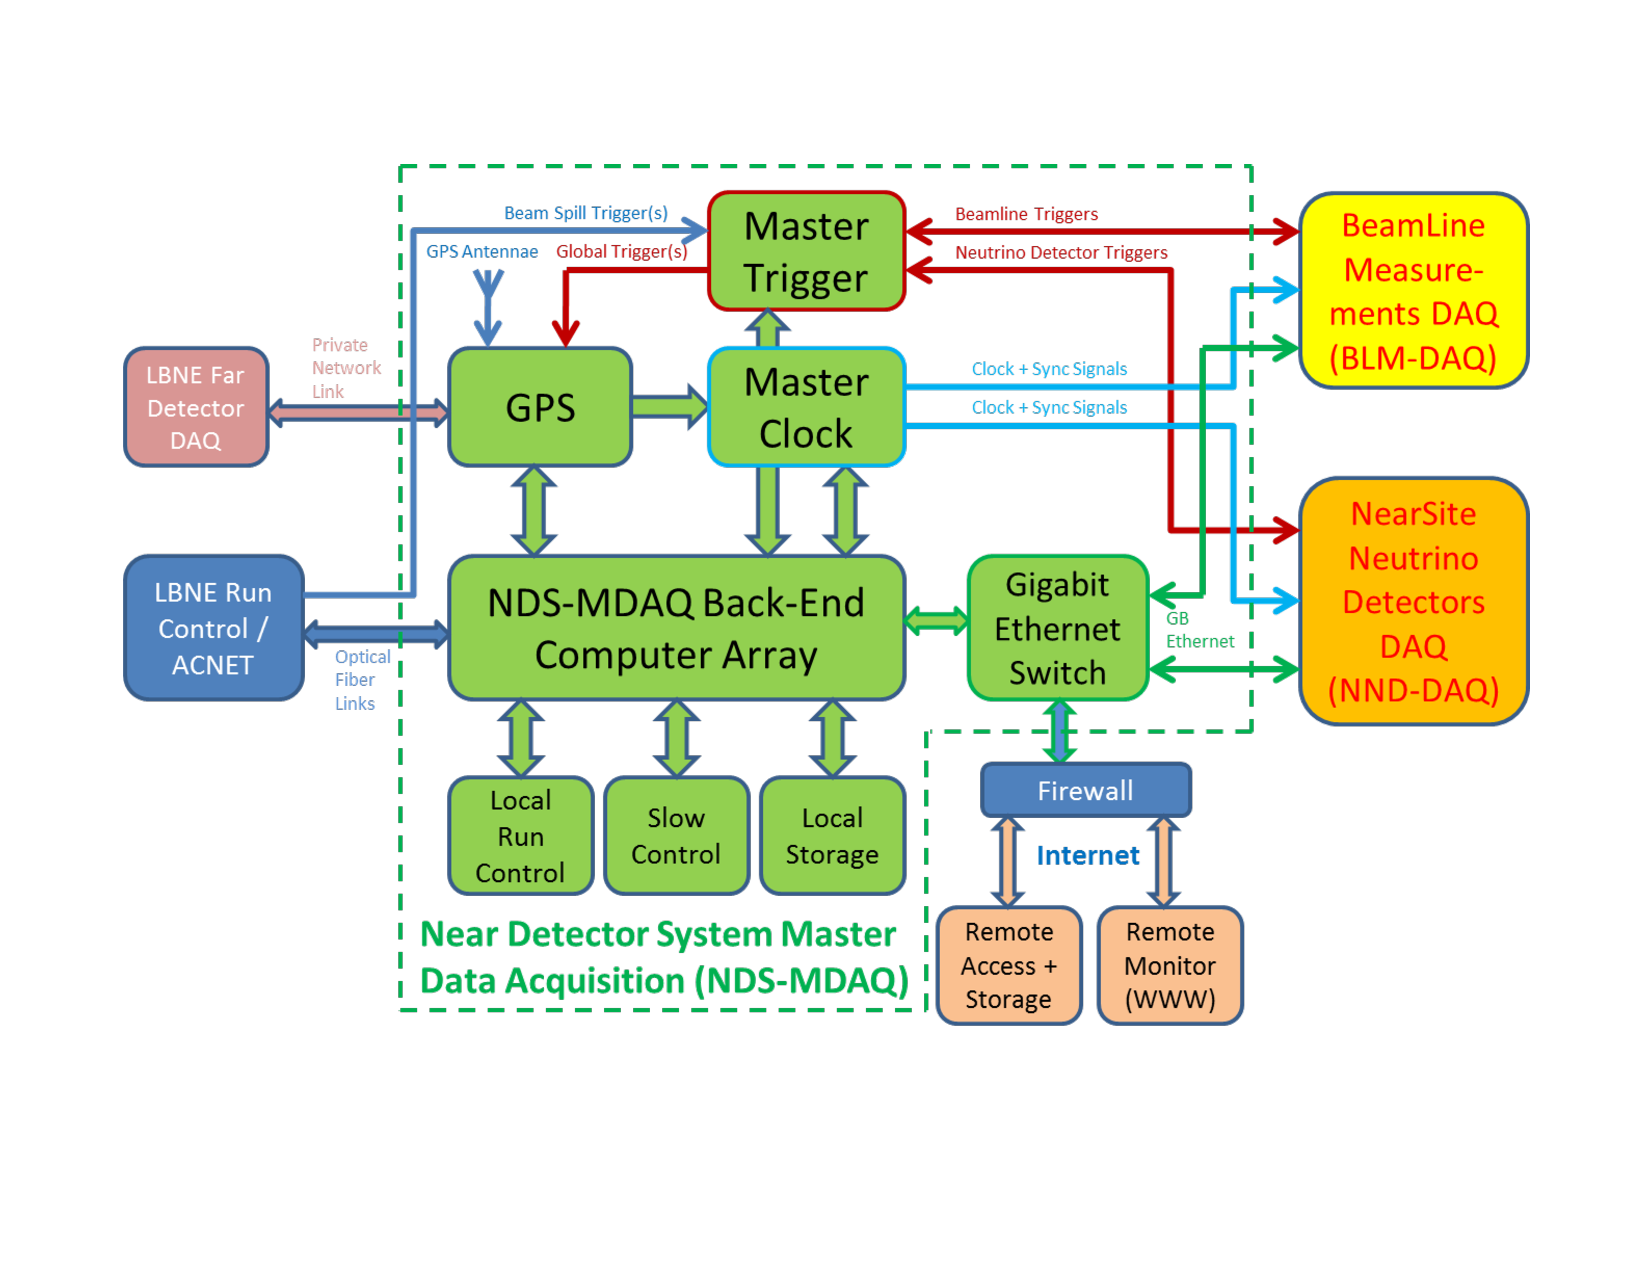
\includegraphics[width=6in,angle=0]{DAQ_Block}
\end{cdrfigure}

\fixme{The labels within the figure still say LBNE, can we fix this?}

The NDS computing system encompasses two major activities: online computing (the required
slow-control systems \fixme{for what systems}) and offline computing for further development of the measurement 
strategy and for simulation work on technical systems. \fixme{why do we say `for further development of'? Why not just 
offline computing and simulation work?  Or is it only a portion of the offline computing?  Probably need to say how it 
interfaces with DUNE computing. Also say how it interfaces with DAQ; there's no connecting text between daq and computing. }

\subsection{NDS Master DAQ} % and Computing}
\label{sec:nd-master-daq}

\fixme{please clarify in this section what is the overall NDS DAQ and what is the master DAQ.}

The NDS-DAQ %design consists of equipment 
is designed to provide a high-level user interface 
for local run control and data taking, as well as for secure remote control and monitoring.   It will 
serve as the primary interface to the 
\begin{itemize}
\item slow-control system 
\item online data and DAQ performance monitoring  
\item raw data collection
\item building of events
\item data storage   
\end{itemize}
between all Near 
Neutrino Detector DAQs and Beamline Measurements DAQs. \fixme{It's not clear to me exactly WHAT is `between all Near 
Neutrino Detector DAQs and Beamline Measurements DAQs.'}

The NDS-DAQ \fixme{check} includes hardware triggering 
for two-way trigger processing between the NDS-DAQ \fixme{the master?} and all the NDS detectors, and 
\fixme{between itself and?} GPS for precision 
time-stamping and global \fixme{global?} clock synchronization.  It \fixme{The design?} is currently based on a channel count 
estimate of approximately 430,000 channels of neutrino detectors, plus $<1,000$ channels of 
beamline detectors.  Custom electronics components for the NDS-DAQ are based on existing 
custom designs from other experiments, e.g,. T2K or ATLAS, \fixme{you can say ``they ARE based on X and Y'' or
``they WILL BE based on X or Y'' but not``they ARE based on X or Y'' } and %have all commercial 
implement commercial components for the trigger modules, clock and timing synchronization, GPS and environmental 
monitoring.

%The computing system encompasses two major activities: online computing with required 
%slow-control systems, and offline computing for further development of the measurement 
%strategy and for simulation work on technical systems. 
%The computing components are based 
%on currently available commercial computing and gigabit networking technology, which is 
%likely to improve over the next years without driving costs up for the final design.  

\fixme{I don't know why this section was for daq and computing. There's no explanation of how one leads
to the other or how they're related (I know they are!)}

\subsection{Near Neutrino Detector DAQ (NND-DAQ)} % Nearsite Neutrino Detector (NND) DAQ}
\label{sec:nd:nnd:daq}

%\fixme{why isn't this called the FGT-DAQ?  It's hard to know whether to use FGT or NND. FGT is easier to keep straight in your mind from NDS, that's for sure!; WCL: we agreed with Hans to use NND-DAQ. Ok AH}

The Near Neutrino Detector Data Acquisition system (NND-DAQ) collects raw data from 
each %near 
detector subsystem in the Near Neutrino Detector (NND) and connects to the (overall) Near 
Detector System DAQ (NDS-DAQ) via Gigabit Ethernet. A block diagram of the NND-DAQ is
shown in Figure~\ref{DAQ_NND}. The NND-DAQ will mainly consist 
of a scalable back-end computer array, inter-connected to the individual Near Neutrino 
Detector DAQs via Gigabit Ethernet, and specialized electronics modules for trigger 
processing and clock synchronization. It interfaces to the NDS Master DAQ (NDS-MDAQ) for 
run control and global data collection. The NND-DAQ will also have its own local run-control setup, 
consisting of a number of desktop workstations to allow independent local runs that include 
nearsite neutrino detectors only, useful during detector commissioning, calibration runs, 
stand-alone cosmic runs, or other runs where the beam is stopped or not needed.

The quantity of computers required for the back-end system is highly dependent on the 
number of channels and expected data rates of the individual neutrino detectors. Based on 
T2K Near Detector DAQ experience\fixme{ref? (not addressed)}, one back-end computer should be able to handle 
approximately 3,000 channels for sustainable and continuous runs. Assuming a total of 
430,000 channels for all NND subdetectors combined, about 150 back-end computers would be 
needed.

Trigger signals from each subdetector will be collected and pre-processed by a 
trigger electronics module, similar in design to the NDS  trigger or master clock modules 
of the NDS-DAQ design. Depending on the run mode, this module could feed local trigger 
decisions to the detector DAQs for data collection, or it could forward NDS triggers 
from the NDS-DAQ or higher levels to the neutrino detector DAQs.  A slave-clock electronics 
module, similar to the master-clock module in the NDS-DAQ, distributes clock- and 
time-synchronization signals from the NDS-DAQ to all NND subdetectors.


\begin{cdrfigure}[A block diagram of the Near Neutrino Detector DAQ]{DAQ_NND}{A block diagram of the Near Neutrino Detector DAQ (NND-DAQ)}
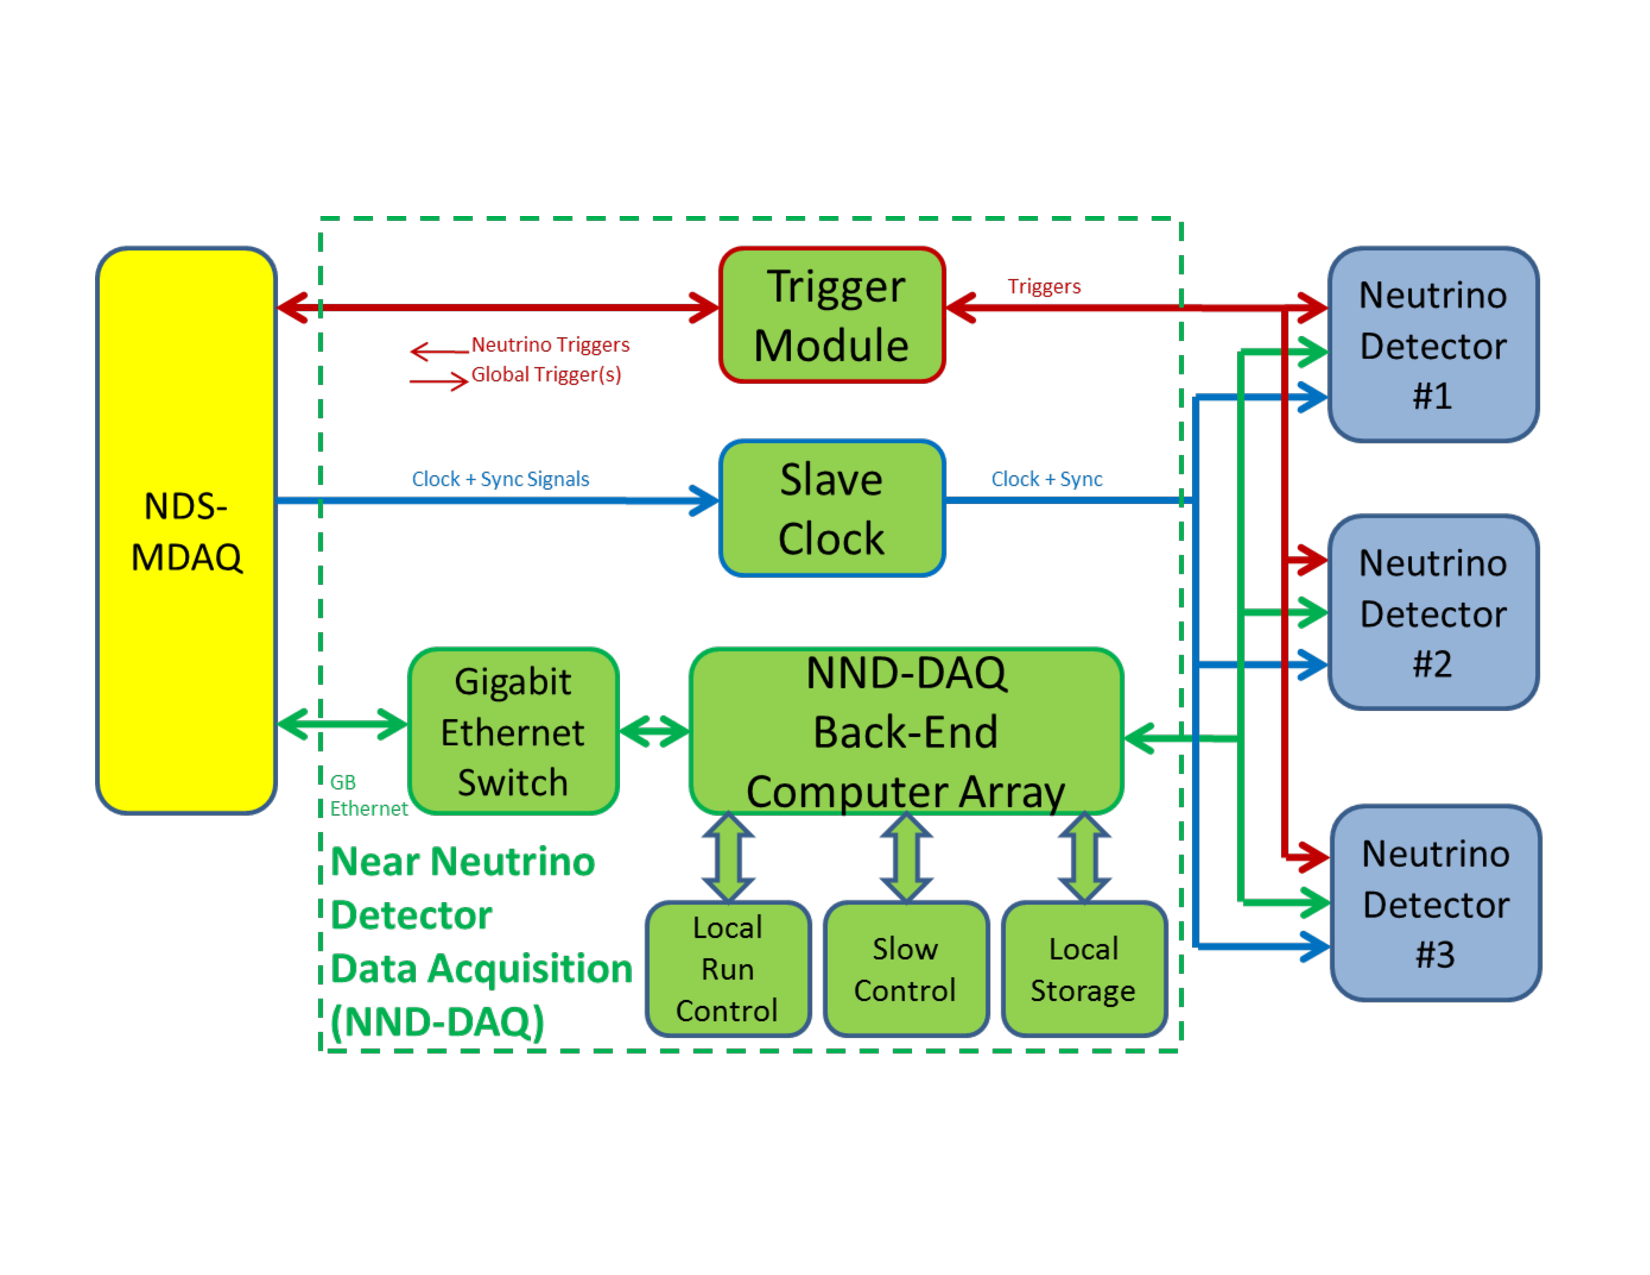
\includegraphics[width=6in,angle=0]{DAQ_NND}
\end{cdrfigure}


\subsection{Beamline Measurements DAQ (BLM-DAQ)}

Similar to the NDS Master DAQ, the BLM-DAQ will mainly consist of a scalable back-end 
computer array, inter-connected to the individual beamline measurement detector DAQs via 
Gigabit Ethernet and specialized electronics modules for trigger processing and clock 
synchronization. 
\fixme{None of this is covered in the master daq section. I suspect that we need to retrieve some info
from the earlier version of this chapter when it was ``global daq''}
It interfaces to the NDS Master DAQ (NDS-MDAQ) for run control and global \fixme{want to use `global'?}
data collection. It will also have its own local run-control setup, consisting of a number 
of desktop workstations to allow independent local runs that include beamline measurement 
detectors only (useful during detector commissioning), calibration runs, stand-alone cosmic 
runs or other runs where the beam is stopped or not needed.


\section{NDS Computing}
\label{sec:nd-gdaq-global-computing}

The computing system encompasses two major activities: online computing with required 
slow-control systems, and offline computing for further development of the measurement 
strategy and for simulation work on technical systems. The computing components are based 
on currently available commercial computing and gigabit networking technology, which is 
likely to improve over the next years without driving costs up for the final design.  
 \fixme{There's no
mention of how the DAQ and the computing system are linked}

